% =============================================================================
%  Diplomado en Data Science Aplicada con Python para la Toma de Decisiones
%  Clase 34: Del LSTM al LLM --- como nacieron los Transformers
%  Arca Continental Ecuador | UDLA
% =============================================================================
\documentclass[aspectratio=169, 11pt]{beamer}

\usepackage[T1]{fontenc}
\usepackage[utf8]{inputenc}
\usepackage[spanish,es-noshorthands]{babel}
\usepackage{FiraSans}
\usepackage{FiraMono}
\renewcommand{\familydefault}{\sfdefault}
\usepackage{graphicx}
\usepackage{tikz}
\usetikzlibrary{arrows.meta, positioning, shapes.geometric, shapes.misc,
  calc, fit, decorations.pathreplacing, backgrounds, matrix, chains}
\usepackage{fontawesome5}
\usepackage{minted}
\usepackage{tcolorbox}
\tcbuselibrary{minted, skins, breakable}
\usepackage{booktabs}
\usepackage{colortbl}
\usepackage{multicol}
\usepackage{hyperref}
\usepackage{calc}
\usepackage{amsmath}

\definecolor{arcaRed}{HTML}{C82B40}
\definecolor{arcaDark}{HTML}{6B1525}
\definecolor{arcaGray}{HTML}{F5F5F5}
\definecolor{arcaLightGray}{HTML}{EBEBEB}
\definecolor{textDark}{HTML}{2D2D2D}
\definecolor{textMuted}{HTML}{6B7280}
\definecolor{codeGreen}{HTML}{16A34A}
\definecolor{codeBlue}{HTML}{2563EB}
\definecolor{codeOrange}{HTML}{EA580C}
\definecolor{codePurple}{HTML}{7C3AED}

\usetheme{default}
\usecolortheme{default}
\setbeamertemplate{navigation symbols}{}
\setbeamertemplate{footline}{}
\setbeamertemplate{headline}{}
\setbeamercolor{normal text}{fg=textDark}
\setbeamercolor{frametitle}{fg=arcaRed, bg=white}
\setbeamercolor{title}{fg=white}
\setbeamercolor{subtitle}{fg=white!85}
\setbeamercolor{author}{fg=white!80}
\setbeamercolor{date}{fg=white!70}
\setbeamercolor{item}{fg=arcaRed}
\setbeamercolor{subitem}{fg=arcaDark}
\setbeamercolor{block title}{fg=white, bg=arcaRed}
\setbeamercolor{block body}{fg=textDark, bg=arcaGray}
\setbeamerfont{frametitle}{size=\Large, series=\bfseries}
\setbeamerfont{title}{size=\huge, series=\bfseries}
\setbeamerfont{subtitle}{size=\large}
\setbeamerfont{author}{size=\normalsize}
\setbeamerfont{date}{size=\small}
\setbeamertemplate{itemize item}{\scriptsize\raise1.5pt\hbox{\color{arcaRed}$\blacktriangleright$}}
\setbeamertemplate{itemize subitem}{\scriptsize\raise1pt\hbox{\color{arcaDark}$\bullet$}}
\setbeamertemplate{enumerate items}[default]
\setbeamercolor{enumerate item}{fg=arcaRed}

\setbeamertemplate{headline}{%
  \begin{tikzpicture}[remember picture, overlay]
    \fill[arcaDark] (current page.north west) rectangle
      ([yshift=-0.7cm]current page.north east);
    \node[anchor=west, inner sep=0pt] at
      ([xshift=0.6cm, yshift=-0.35cm]current page.north west)
      {
\includegraphics[height=0.45cm]{../logo_udla_white.png}};
    \node[anchor=east, inner sep=0pt] at
      ([xshift=-0.6cm, yshift=-0.35cm]current page.north east)
      {
\includegraphics[height=0.45cm]{../ArcaContinental_white.png}};
  \end{tikzpicture}%
  \vspace{0.7cm}%
}

\setbeamertemplate{footline}{%
  \begin{tikzpicture}[remember picture, overlay]
    \node[anchor=south east, font=\scriptsize\bfseries\color{arcaRed}] at
      ([xshift=-0.5cm, yshift=0.15cm]current page.south east)
      {\insertframenumber};
  \end{tikzpicture}%
  \vspace{0.3cm}%
}

\setbeamertemplate{frametitle}{%
  \vspace{0.25cm}%
  \usebeamerfont{frametitle}\usebeamercolor[fg]{frametitle}\insertframetitle%
  \par\vspace{2pt}%
  \begin{tikzpicture}
    \fill[arcaRed] (0,0) rectangle (3cm, 1.5pt);
    \fill[arcaLightGray] (3cm,0) rectangle (\textwidth, 0.5pt);
  \end{tikzpicture}%
  \vspace{0.1cm}%
}

\newtcblisting{pyblock}[1][]{%
  listing engine=minted, minted language=python, minted style=friendly,
  minted options={fontsize=\small, linenos=false, breaklines=true, python3=true},
  colback=arcaGray, colframe=arcaRed, left=4pt, right=4pt, top=4pt, bottom=4pt,
  boxrule=0pt, leftrule=3pt, arc=2pt, listing only, #1}

\newcommand{\sectionframe}[2]{%
  \begingroup
  \setbeamertemplate{headline}{}%
  \setbeamertemplate{footline}{}%
  \begin{frame}[plain, noframenumbering]
    \begin{tikzpicture}[remember picture, overlay]
      \fill[arcaRed] (current page.south west) rectangle (current page.north east);
      \node[anchor=center, text=white, font=\Huge\bfseries, text width=12cm,
            align=center] at ([yshift=0.5cm]current page.center) {#1};
      \node[anchor=center, text=white!80, font=\large, text width=10cm,
            align=center] at ([yshift=-0.8cm]current page.center) {#2};
    \end{tikzpicture}
  \end{frame}
  \endgroup
}

% --- estilos TikZ reutilizables ---
\tikzset{
  arrowR/.style={-{Stealth[length=2.5mm]}, arcaRed, thick},
  arrowD/.style={-{Stealth[length=2.5mm]}, arcaDark, thick},
  arrowG/.style={-{Stealth[length=2.5mm]}, color=textMuted, thick, dashed},
  boxA/.style={rectangle, rounded corners=4pt, draw=arcaDark, fill=arcaGray,
               align=center, font=\footnotesize, inner sep=4pt, minimum height=0.9cm},
  boxRed/.style={rectangle, rounded corners=4pt, draw=arcaDark, fill=arcaRed,
                 text=white, align=center, font=\bfseries\footnotesize,
                 inner sep=5pt, minimum height=0.9cm},
  boxBlue/.style={rectangle, rounded corners=4pt, draw=arcaDark, fill=codeBlue,
                  text=white, align=center, font=\bfseries\footnotesize,
                  inner sep=5pt, minimum height=0.9cm},
  boxGreen/.style={rectangle, rounded corners=4pt, draw=arcaDark, fill=codeGreen,
                   text=white, align=center, font=\bfseries\footnotesize,
                   inner sep=5pt, minimum height=0.9cm},
  boxOrange/.style={rectangle, rounded corners=4pt, draw=arcaDark, fill=codeOrange,
                    text=white, align=center, font=\bfseries\footnotesize,
                    inner sep=5pt, minimum height=0.9cm},
}

\title{Diplomado en Data Science Aplicada\\con Python para la Toma de Decisiones}
\subtitle{Clase 34: Del LSTM al LLM --- cómo nacieron los Transformers}
\author{Carlos Enrique Mosquera Trujillo}
\date{30 de Mayo, 2026}

\begin{document}

% ===================== PORTADA =====================
{
\setbeamertemplate{headline}{}
\setbeamertemplate{footline}{}
\begin{frame}[plain, noframenumbering]
  \begin{tikzpicture}[remember picture, overlay]
    \fill[arcaDark] (current page.south west) rectangle (current page.north east);
    \fill[arcaRed] ([yshift=-3.5cm]current page.north west) rectangle
      ([yshift=-4.2cm]current page.north east);
    \node[anchor=west, inner sep=0pt] at
      ([xshift=1cm, yshift=-1.5cm]current page.north west)
      {
\includegraphics[height=1cm]{../logo_udla_white.png}};
    \node[anchor=east, inner sep=0pt] at
      ([xshift=-1cm, yshift=-1.5cm]current page.north east)
      {
\includegraphics[height=1cm]{../ArcaContinental_white.png}};
  \end{tikzpicture}
  \vspace{2.5cm}
  \begin{center}
    {\usebeamerfont{title}\usebeamercolor[fg]{title}\inserttitle\par}
    \vspace{0.4cm}
    {\usebeamerfont{subtitle}\usebeamercolor[fg]{subtitle}\insertsubtitle\par}
    \vspace{0.6cm}
    {\usebeamerfont{author}\usebeamercolor[fg]{author}\insertauthor\par}
    \vspace{0.15cm}
    {\usebeamerfont{date}\usebeamercolor[fg]{date}\insertdate\par}
  \end{center}
\end{frame}
}

% ===================== APERTURA =====================
\sectionframe{Apertura}{De las secuencias al lenguaje:\\cerramos series, abrimos los Transformers}

\begin{frame}[shrink]{Dónde quedamos en la clase 33}
  \vspace{4pt}
  {\footnotesize\color{arcaDark}En la clase pasada construimos la \textbf{escalera de representación}:\par}
  \vspace{6pt}
  \begin{center}
  \begin{tikzpicture}[node distance=0.4cm and 0.5cm, font=\scriptsize]
    \node[boxA, fill=codeBlue!20]    (b) {1. Bag-of-Words\\contar palabras};
    \node[boxA, fill=codeOrange!20, right=of b]  (t) {2. TF-IDF\\pesar por rareza};
    \node[boxA, fill=codeGreen!20, right=of t]   (e) {3. Word2Vec\\significado = vector};
    \node[boxA, fill=codePurple!20, right=of e]  (a) {4. Atención\\significado en contexto};
    \draw[arrowR] (b) -- (t); \draw[arrowR] (t) -- (e); \draw[arrowR] (e) -- (a);
    \node[below=0.1cm of a, font=\tiny\itshape\color{arcaRed}, align=center]
      {\faClock~paramos aquí};
  \end{tikzpicture}
  \end{center}
  \vspace{8pt}
  \begin{tcolorbox}[colback=arcaGray, colframe=arcaRed, leftrule=3pt,
    boxrule=0pt, sharp corners, left=8pt, right=8pt, top=4pt, bottom=4pt]
    {\footnotesize\color{arcaDark}
    Vimos que TF-IDF+LogReg llega a \textbf{84\%} en sentimiento, pero falla con
    frases como \textit{``no me gustó nada''}: el conteo no ve el orden ni la negación.
    Cerramos con la \textbf{idea} de atención. Hoy entendemos cómo funciona por dentro
    y de dónde salieron los LLMs.}
  \end{tcolorbox}
\end{frame}

\begin{frame}[shrink]{La pregunta del día}
  \vspace{14pt}
  \begin{center}
  \begin{tcolorbox}[colback=arcaDark, colframe=arcaDark, sharp corners,
    boxrule=0pt, left=14pt, right=14pt, top=10pt, bottom=10pt, width=0.92\textwidth]
    {\large\color{white}\bfseries
    ¿Cómo le enseñamos a una máquina a entender el lenguaje de Arca
    --- manuales de mantenimiento, tickets de planta, quejas de consumidor ---
    sin contratar 50 lingüistas?\par}
  \end{tcolorbox}
  \end{center}
  \vspace{14pt}
  \begin{itemize}\setlength{\itemsep}{4pt}
    \footnotesize
    \item Es una pregunta vieja. Las primeras respuestas (RNN, LSTM) funcionaron a medias.
    \item En 2017 cambió todo con un paper de 8 personas en Google.
    \item Hoy la respuesta práctica son los \textbf{LLMs pre-entrenados}: no los entrenas, los usas.
  \end{itemize}
  \vspace{6pt}
  \begin{tcolorbox}[colback=arcaRed!8, colframe=arcaRed, leftrule=3pt,
    boxrule=0pt, sharp corners, left=8pt, right=8pt, top=4pt, bottom=4pt]
    {\footnotesize\color{arcaDark}\bfseries
    Esta pregunta nos acompaña en los 4 bloques. Cada bloque es una respuesta cada vez mejor.}
  \end{tcolorbox}
\end{frame}

\begin{frame}[shrink]{El arco de hoy --- de Cervantes a ChatGPT}
  \begin{center}
  \begin{tikzpicture}[node distance=0.35cm and 0.4cm, font=\scriptsize]
    \node[boxBlue]   (rnn)  {RNN / LSTM\\1986--2016};
    \node[boxRed, right=of rnn]    (trf)  {Transformer\\2017};
    \node[boxOrange, right=of trf] (gpt2) {GPT-2 / BERT\\2018--2019};
    \node[boxGreen, right=of gpt2]  (gpt) {GPT-3 / ChatGPT\\2020--2022};
    \node[fill=arcaDark, text=white, rounded corners=4pt, font=\bfseries\footnotesize,
          inner sep=5pt, minimum height=0.9cm, align=center, right=of gpt] (llm) {Claude / GPT-5\\2024--2026};
    \draw[arrowR] (rnn) -- (trf); \draw[arrowR] (trf) -- (gpt2);
    \draw[arrowR] (gpt2) -- (gpt); \draw[arrowR] (gpt) -- (llm);
  \end{tikzpicture}
  \end{center}
  \vspace{10pt}
  \begin{enumerate}\setlength{\itemsep}{4pt}
    \footnotesize
    \item[\textbf{1.}] \textbf{Antes del Transformer} --- RNN/LSTM, sus 3 muros, y un LSTM real escribiendo Quijote.
    \item[\textbf{2.}] \textbf{2017: ``Attention is All You Need''} --- la idea, Query-Key-Value, multi-head.
    \item[\textbf{3.}] \textbf{Mini-Transformer en acción} --- desde cero fracasa, pre-entrenado (BETO) ya entiende la negación.
    \item[\textbf{4.}] \textbf{LLMs en la práctica} --- panorámica del ecosistema y demo real con Groq en 5 líneas.
  \end{enumerate}
  \vspace{4pt}
  \begin{tcolorbox}[colback=arcaRed!8, colframe=arcaRed, leftrule=3pt,
    boxrule=0pt, sharp corners, left=8pt, right=8pt, top=3pt, bottom=3pt]
    {\footnotesize\color{arcaDark}\bfseries
    Hoy entendemos cómo funcionan. El \emph{hands-on profundo} (prompting, RAG,
    agentes, scraping) es el Módulo 6.}
  \end{tcolorbox}
\end{frame}

% =============================================================================
%  BLOQUE 1 - ANTES DEL TRANSFORMER
% =============================================================================
\sectionframe{Bloque 1}{Antes del Transformer:\\RNN, LSTM y sus tres muros}

\begin{frame}[shrink]{El problema del texto para una red normal}
  \vspace{4pt}
  \begin{tcolorbox}[colback=arcaGray, colframe=arcaRed, leftrule=3pt,
    boxrule=0pt, sharp corners, left=8pt, right=8pt, top=6pt, bottom=6pt]
    {\footnotesize\color{arcaDark}
    Una red densa (la del Módulo 4) espera \textbf{una entrada de tamaño fijo}.
    El texto no es así: una frase tiene 5 palabras, otra 200; \textbf{el orden importa}
    (\textit{``perro muerde hombre''} $\neq$ \textit{``hombre muerde perro''}); y la
    misma palabra significa cosas distintas según el contexto.}
  \end{tcolorbox}
  \vspace{8pt}
  \begin{center}
  \begin{tikzpicture}[node distance=0.5cm, font=\footnotesize]
    \node[boxA] (x1) {$x_1$};
    \node[boxA, right=of x1] (x2) {$x_2$};
    \node[boxA, right=of x2] (x3) {$x_3$};
    \node[font=\Large, right=of x3] (dots) {$\cdots$};
    \node[boxA, right=of dots] (xn) {$x_n$};
    \node[below=0.1cm of x1, font=\tiny\itshape\color{textMuted}] {``el''};
    \node[below=0.1cm of x2, font=\tiny\itshape\color{textMuted}] {``compresor''};
    \node[below=0.1cm of x3, font=\tiny\itshape\color{textMuted}] {``vibra''};
    \node[below=0.1cm of xn, font=\tiny\itshape\color{textMuted}] {``raro''};
    \node[above=0.4cm of x2, font=\footnotesize, color=arcaDark] (q) {¿cómo procesar esto en orden, sin perder lo que viene atrás?};
    \draw[arrowG] (q) -- (x2);
  \end{tikzpicture}
  \end{center}
  \vspace{6pt}
  {\footnotesize\color{arcaDark}
  La solución de los 90s/00s: una red que lee la secuencia \textbf{paso a paso} con memoria.}
\end{frame}

\begin{frame}[shrink]{La RNN --- una neurona con memoria, desplegada en el tiempo}
  \begin{center}
  \begin{tikzpicture}[node distance=0.6cm and 0.7cm, font=\footnotesize]
    \foreach \i/\w in {1/el,2/compresor,3/vibra,4/raro} {
      \node[boxA, fill=codeBlue!20] (x\i) at (\i*2.5, 0) {$x_{\i}$};
      \node[below=0.05cm of x\i, font=\tiny\itshape\color{textMuted}] {\w};
      \node[boxRed, above=0.8cm of x\i] (h\i) {RNN};
      \node[boxGreen, above=0.7cm of h\i] (y\i) {$h_{\i}$};
      \draw[arrowR] (x\i) -- (h\i);
      \draw[arrowR] (h\i) -- (y\i);
    }
    \foreach \i/\j in {1/2,2/3,3/4} {
      \draw[arrowD] (h\i) -- node[above, font=\tiny] {memoria} (h\j);
    }
    \node[font=\scriptsize\itshape\color{arcaDark}, below=1.3cm of x1.south west,
          anchor=west, align=left, text width=14cm]
      {Cada paso recibe el dato actual $x_t$ y la memoria del paso anterior.
       En teoría \textbf{recuerda todo el pasado}; en la práctica, los gradientes
       se desvanecen y olvida tras pocos pasos.};
  \end{tikzpicture}
  \end{center}
\end{frame}

\begin{frame}[shrink]{La LSTM --- el upgrade de la RNN (1997)}
  \begin{columns}[c]
    \begin{column}{0.50\textwidth}
      \begin{tcolorbox}[colback=arcaGray, colframe=arcaRed, leftrule=3pt,
        boxrule=0pt, sharp corners, left=8pt, right=8pt, top=4pt, bottom=4pt]
        {\footnotesize\color{arcaDark}
        Una \textbf{LSTM} (Long Short-Term Memory) le agrega \textbf{compuertas}
        a la RNN para decidir qué olvidar, qué recordar y qué devolver.\par
        \vspace{4pt}
        Resuelve el problema de la memoria corta de las RNN: puede recordar
        algo de cien pasos atrás \emph{si} aprende que vale la pena.}
      \end{tcolorbox}
    \end{column}
    \begin{column}{0.48\textwidth}
      \begin{center}
      \begin{tikzpicture}[font=\scriptsize, node distance=0.3cm]
        \node[boxBlue] (x) {$x_t$};
        \node[boxRed, right=1.2cm of x, minimum width=2.5cm, minimum height=1.5cm]
              (c) {LSTM cell\\\tiny\bfseries (olvidar/recordar)};
        \node[boxGreen, right=1.2cm of c] (h) {$h_t$};
        \draw[arrowR] (x) -- (c);
        \draw[arrowR] (c) -- (h);
        \draw[arrowD, dashed] (c.south) to[bend right=30] node[below, font=\tiny]
          {memoria a $t+1$} ($(c.south)+(2.5,-0.6)$);
      \end{tikzpicture}
      \end{center}
    \end{column}
  \end{columns}
  \vspace{8pt}
  {\footnotesize\color{arcaDark}
  Las LSTM fueron \textbf{el modelo dominante del NLP entre 2014 y 2017}.
  Google Translate, Siri, autocompletar de teclado --- todos eran LSTMs.}
\end{frame}

\begin{frame}[shrink]{De clasificar a GENERAR --- la idea del char-LSTM}
  \vspace{4pt}
  \begin{center}
  \begin{tikzpicture}[font=\footnotesize, node distance=0.4cm]
    \node[boxA] (a) {``en un lugar de la manch''};
    \node[boxRed, right=1cm of a] (l) {LSTM};
    \node[boxGreen, right=1cm of l] (p) {siguiente: ``a''};
    \draw[arrowR] (a) -- (l);
    \draw[arrowR] (l) -- (p);
    \draw[->, >=Stealth, color=codeGreen, thick, line width=1.2pt]
      (p.south) to[bend left=45]
      node[below=2pt, font=\scriptsize\itshape\color{codeGreen}]
      {realimentar y repetir $\Rightarrow$ escribe la frase entera}
      (a.south);
  \end{tikzpicture}
  \end{center}
  \vspace{6pt}
  \begin{tcolorbox}[colback=arcaRed!8, colframe=arcaRed, leftrule=3pt,
    boxrule=0pt, sharp corners, left=8pt, right=8pt, top=6pt, bottom=6pt]
    {\small\color{arcaDark}
    La receta de la \textbf{generación}: predecir el siguiente elemento, agregarlo
    a la secuencia, repetir. Así la red \emph{escribe sola}, carácter por carácter.\par
    \vspace{2pt}
    \textbf{Una red densa o una CNN no pueden hacer esto}: necesitan ver toda la
    entrada de una vez. Generar requiere memoria del pasado --- y la LSTM la tiene.}
  \end{tcolorbox}
\end{frame}

\begin{frame}[fragile, shrink]{El código --- char-LSTM en 8 líneas de Keras}
  \begin{pyblock}
import tensorflow as tf
from tensorflow.keras import layers, Sequential, Input

SEQ = 60                                  # ventana de 60 caracteres
model = Sequential([
    Input((SEQ,)),
    layers.Embedding(vocab_size, 64),     # cada caracter a vector
    layers.LSTM(256),                     # la memoria
    layers.Dense(vocab_size),             # probabilidad del siguiente caracter
])
model.compile("adam", loss=tf.keras.losses.SparseCategoricalCrossentropy(from_logits=True))
model.fit(X, y, epochs=10)                # X = ventanas, y = siguiente caracter
  \end{pyblock}
  \vspace{4pt}
  {\footnotesize\color{arcaDark}
  Entrenamos sobre \textbf{Don Quijote} (2~MB) en GPU. En $\sim$2 minutos aprende
  ortografía, palabras y sintaxis del español. \emph{Nadie le dijo nada} --- solo a
  predecir el siguiente carácter.}
\end{frame}

\begin{frame}[shrink]{Aprende español desde cero (la curva real)}
  \begin{center}
    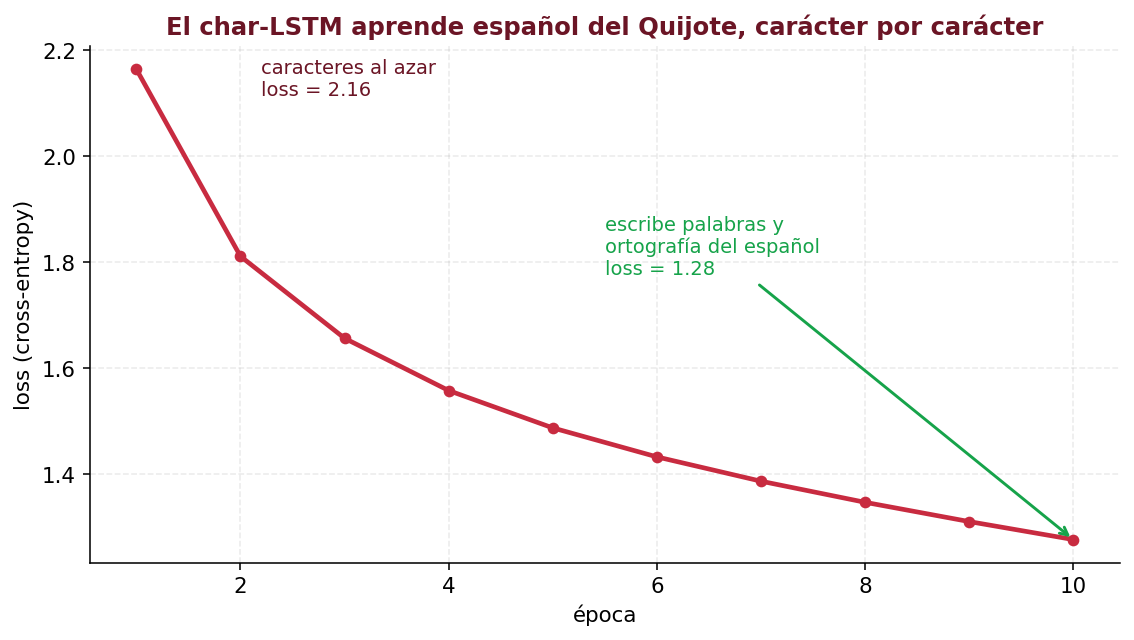
\includegraphics[width=0.78\textwidth]{fig_charlstm_loss.png}
  \end{center}
  \vspace{2pt}
  {\footnotesize\color{arcaDark}
  De \textbf{loss 2.96 a 1.28} en 10 épocas. La red descubre sola que algunas
  letras siguen a otras, que las palabras se separan con espacios, y que después
  del punto viene mayúscula.}
\end{frame}

\begin{frame}[shrink]{Lo que escribe el char-LSTM --- 3 temperaturas}
  \vspace{2pt}
  \begin{tcolorbox}[colback=arcaGray, colframe=arcaDark, leftrule=2pt,
    boxrule=0pt, sharp corners, left=8pt, right=8pt, top=4pt, bottom=4pt,
    title={\footnotesize\color{white}\bfseries temperatura 0.4 \;\faSnowflake},
    coltitle=white, colbacktitle=arcaDark, fonttitle=\footnotesize]
    {\footnotesize\itshape\color{textDark}
    en un lugar de la mancha de cuyo nombre no quiero acordarme al caballero
    andante se le ha de ser aquel sancho que se la había de ver esperador de la
    mancha, que se me ha de ser aquel alcanceciaron las caballerías...}
  \end{tcolorbox}
  \vspace{4pt}
  \begin{tcolorbox}[colback=arcaGray, colframe=arcaDark, leftrule=2pt,
    boxrule=0pt, sharp corners, left=8pt, right=8pt, top=4pt, bottom=4pt,
    title={\footnotesize\color{white}\bfseries temperatura 0.8 \;\faBalanceScale},
    coltitle=white, colbacktitle=arcaDark, fonttitle=\footnotesize]
    {\footnotesize\itshape\color{textDark}
    en un lugar de la mancha de cuyo nombre no quiero acordarme al cura por
    adadustedo. sancho de aquella veza a bastar se les refunta señora, y que
    aquella le podía agrada que nos casados...}
  \end{tcolorbox}
  \vspace{4pt}
  \begin{tcolorbox}[colback=arcaGray, colframe=arcaDark, leftrule=2pt,
    boxrule=0pt, sharp corners, left=8pt, right=8pt, top=4pt, bottom=4pt,
    title={\footnotesize\color{white}\bfseries temperatura 1.2 \;\faFire},
    coltitle=white, colbacktitle=arcaDark, fonttitle=\footnotesize]
    {\footnotesize\itshape\color{textDark}
    en un lugar de la mancha de cuyo nombre no quiero acordarme a enasmora lenga
    de los baldanes plómezos botos sancho panza, madóndese el truerte que se
    dijeron; que nos más viejos y abrianos...}
  \end{tcolorbox}
  \vspace{4pt}
  {\footnotesize\color{arcaDark}
  Imperfecto, pero \textbf{aprendió la estructura del español sin instrucciones}.
  El \textbf{techo pre-Transformer} era esto. \textbf{GPT hace exactamente lo mismo}
  --- predecir el siguiente token --- pero con atención y a otra escala.}
\end{frame}

\begin{frame}[shrink]{Seq2seq --- traducción, resumen, diálogo (Sutskever, 2014)}
  \begin{center}
  \begin{tikzpicture}[node distance=0.5cm, font=\footnotesize]
    % entrada (3 palabras en EN)
    \foreach \i/\w in {1/I,2/love,3/you} {
      \node[boxA, fill=codeBlue!20, minimum width=1.4cm]
        (e\i) at (\i*1.6, 0) {\w};
    }
    % encoder
    \node[boxRed, above=0.6cm of e2, minimum width=5cm] (enc) {ENCODER LSTM};
    % vector cuello-botella
    \node[fill=arcaDark, text=white, rounded corners=4pt, above=0.5cm of enc,
          minimum width=2.4cm, minimum height=0.9cm, font=\bfseries\scriptsize,
          align=center]
          (z) {vector resumen};
    % decoder
    \node[boxRed, above=0.5cm of z, minimum width=5cm] (dec) {DECODER LSTM};
    % salida (3 palabras en ES) -- centradas SOBRE el decoder, dentro del slide
    \foreach \i/\w in {1/te,2/quiero,3/mucho} {
      \node[boxA, fill=codeGreen!20, minimum width=1.4cm]
        (d\i) at (\i*1.6, \i*0+6.4) {\w};
    }
    % flechas hacia arriba
    \foreach \i in {1,2,3} { \draw[arrowR] (e\i.north) -- (enc.south-|e\i); }
    \draw[arrowR] (enc.north) -- (z.south);
    \draw[arrowR] (z.north) -- (dec.south);
    \foreach \i in {1,2,3} { \draw[arrowR] (dec.north-|d\i) -- (d\i.south); }
  \end{tikzpicture}
  \end{center}
  \vspace{8pt}
  {\footnotesize\color{arcaDark}
  El \textbf{encoder} (LSTM 1) comprime la frase en un \textbf{vector resumen}.
  El \textbf{decoder} (LSTM 2) toma ese vector y genera la traducción token a token.
  Esta arquitectura es la que usaba \textbf{Google Translate antes de 2017}.}
\end{frame}

\begin{frame}[shrink]{Muro 1 --- es secuencial y no paraleliza}
  \vspace{2pt}
  \begin{center}
  \begin{tikzpicture}[font=\footnotesize, node distance=0.3cm]
    \node[font=\scriptsize\bfseries\color{arcaDark}] at (-2.5, 2.6) {LSTM};
    \foreach \i in {1,...,7} {
      \node[boxRed, minimum width=0.7cm, minimum height=0.5cm] (l\i) at (\i*0.9, 2.5) {};
    }
    \foreach \i/\j in {1/2,2/3,3/4,4/5,5/6,6/7} {
      \draw[arrowD] (l\i.east) -- (l\j.west);
    }
    \node[right=0.4cm of l7, font=\scriptsize\color{arcaRed}] {\faClock~lento};

    \node[font=\scriptsize\bfseries\color{arcaDark}] at (-2.5, 0.5) {Transformer};
    \foreach \i in {1,...,7} {
      \node[boxGreen, minimum width=0.7cm, minimum height=0.5cm] (t\i) at (\i*0.9, 0.5) {};
    }
    \draw[decorate, decoration={brace, amplitude=4pt, mirror},color=codeGreen, thick]
      (t1.south west) -- (t7.south east) node[midway, below=4pt, font=\scriptsize]
      {todos a la vez};
    \node[right=0.4cm of t7, font=\scriptsize\color{codeGreen}] {\faRocket~paralelo};
  \end{tikzpicture}
  \end{center}
  \vspace{8pt}
  {\footnotesize\color{arcaDark}
  La LSTM \emph{debe} esperar al paso anterior para procesar el siguiente.
  La GPU está parada el 90\% del tiempo. \textbf{Esto bloquea el escalado.}}
\end{frame}

\begin{frame}[shrink]{Muro 2 --- el cuello de botella del encoder}
  \begin{center}
  \begin{tikzpicture}[font=\footnotesize, node distance=0.4cm]
    \foreach \i/\w in {1/la,2/presión,3/del,4/compresor,5/subió} {
      \node[rectangle, rounded corners=3pt, draw=arcaDark, fill=codeBlue!20,
            minimum width=1.5cm, minimum height=0.7cm, font=\scriptsize]
        (w\i) at (\i*1.7, 0) {\w};
    }
    \node[fill=arcaDark, text=white, rounded corners=4pt, font=\bfseries\footnotesize,
          minimum width=2.2cm, minimum height=1cm, align=center] (z) at (12.5, 0)
          {un\\vector};
    \draw[->, >=Stealth, color=arcaRed, line width=2pt] (w5.east) -- (z.west);
    \node[font=\scriptsize\itshape\color{arcaDark}] at ($(w5.east)!0.5!(z.west)+(0,0.6)$)
          {todo $\to$ un solo vector};
  \end{tikzpicture}
  \end{center}
  \vspace{10pt}
  \begin{tcolorbox}[colback=arcaRed!8, colframe=arcaRed, leftrule=3pt,
    boxrule=0pt, sharp corners, left=8pt, right=8pt, top=4pt, bottom=4pt]
    {\footnotesize\color{arcaDark}\bfseries
    En textos largos, lo que la LSTM leyó al principio queda diluido cuando
    llega al final. Para traducir un párrafo entero, ese ``vector resumen'' es
    insuficiente. La memoria a largo plazo tiene techo.}
  \end{tcolorbox}
\end{frame}

\begin{frame}[shrink]{Muro 3 --- no escala}
  \vspace{4pt}
  \begin{itemize}\setlength{\itemsep}{6pt}
    \footnotesize
    \item \textbf{Datos:} para entrenar bien, una LSTM necesita orden de millones de
    frases etiquetadas. Conseguir esos datos es caro y lento.
    \item \textbf{Cómputo:} su naturaleza secuencial \emph{nulifica} las GPUs modernas.
    Doblar el modelo dobla el tiempo, no rinde más.
    \item \textbf{Resultado:} entre 2014 y 2017, hubo \textbf{techo} en NLP. Google
    Translate mejoraba 1\% por año. Nadie veía cómo salir.
  \end{itemize}
  \vspace{8pt}
  \begin{tcolorbox}[colback=arcaGray, colframe=arcaRed, leftrule=3pt,
    boxrule=0pt, sharp corners, left=8pt, right=8pt, top=6pt, bottom=6pt]
    {\small\color{arcaDark}
    La pregunta que se hicieron en Google en 2017: \emph{¿y si nos olvidamos de la
    recurrencia por completo? ¿y si dejamos que cada palabra mire a todas las demás
    a la vez?}\par}
    \vspace{2pt}
    {\small\color{arcaDark}\bfseries Eso es la atención. Y eso es la siguiente diapositiva.}
  \end{tcolorbox}
\end{frame}

\begin{frame}[shrink]{\faIndustry\ ¿Qué me llevo a Arca? --- Bloque 1}
  \vspace{4pt}
  {\footnotesize\color{arcaDark}\bfseries El lunes ya puedes:\par}
  \vspace{4pt}
  \begin{itemize}\setlength{\itemsep}{4pt}
    \footnotesize
    \item Si Mantenimiento te pide \textbf{autocompletar descripciones recurrentes} de
    tickets (compresor, llenadora, etiquetadora), un \textbf{LSTM chico} entrenado sobre
    2 años de historial es viable y corre en CPU.
    \item \textbf{NO uses LSTM para entender contexto} en quejas de consumidor
    (sarcasmo, negación): el \emph{muro 2} (cuello de botella) te va a morder.
    \item Regla de bolsillo: si tu problema es \textbf{predecir el siguiente paso de una
    secuencia corta y repetitiva}, una LSTM es suficiente y barata. Si necesitas
    contexto largo, no.
  \end{itemize}
  \vspace{6pt}
  \begin{tcolorbox}[colback=arcaGray, colframe=arcaRed, leftrule=3pt,
    boxrule=0pt, sharp corners, left=8pt, right=8pt, top=4pt, bottom=4pt]
    {\footnotesize\color{arcaDark}\bfseries
    Nuestra pregunta: \emph{¿cómo entender el lenguaje de Arca sin contratar 50 lingüistas?}
    \faArrowRight\;Segunda respuesta (siguiente bloque): que cada palabra mire a todas
    a la vez. Eso desbloquea todo.}
  \end{tcolorbox}
\end{frame}

% =============================================================================
%  BLOQUE 2 - ATTENTION IS ALL YOU NEED
% =============================================================================
\sectionframe{Bloque 2}{2017: ``Attention is All You Need''\\el paper que cambió todo}

\begin{frame}[shrink]{Junio 2017 --- un paper de 8 personas en Google Brain}
  \vspace{2pt}
  \begin{center}
  \begin{tcolorbox}[colback=arcaDark, colframe=arcaDark, sharp corners,
    left=14pt, right=14pt, top=10pt, bottom=10pt, width=0.82\textwidth]
    {\Large\color{white}\bfseries Attention is All You Need\par}
    \vspace{4pt}
    {\footnotesize\color{white!85}Vaswani, Shazeer, Parmar, Uszkoreit, Jones, Gomez, Kaiser, Polosukhin\par}
    {\footnotesize\color{white!70}Google Brain --- NeurIPS 2017\par}
  \end{tcolorbox}
  \end{center}
  \vspace{10pt}
  \begin{itemize}\setlength{\itemsep}{4pt}
    \footnotesize
    \item Uno de los \textbf{papers más citados de la historia} de la computación
    (más de 150.000 citas a 2026).
    \item Propone el \textbf{Transformer}: una arquitectura que \emph{elimina la recurrencia
    por completo} y se basa solo en \textbf{atención}.
    \item Es el ancestro de \textbf{GPT, BERT, Claude, Gemini, Llama} --- literalmente
    todos los modelos de lenguaje modernos descienden de aquí.
  \end{itemize}
  \vspace{4pt}
  \begin{tcolorbox}[colback=arcaRed!8, colframe=arcaRed, leftrule=3pt,
    boxrule=0pt, sharp corners, left=8pt, right=8pt, top=3pt, bottom=3pt]
    {\footnotesize\color{arcaDark}\bfseries
    Si solo te llevas un nombre de toda esta clase, que sea este. Aquí empieza
    la era del GenAI.}
  \end{tcolorbox}
\end{frame}

\begin{frame}[shrink]{La idea radical en una frase}
  \vspace{12pt}
  \begin{center}
  \begin{tcolorbox}[colback=arcaGray, colframe=arcaRed, sharp corners,
    leftrule=4pt, boxrule=0pt, left=14pt, right=14pt, top=10pt, bottom=10pt,
    width=0.85\textwidth]
    {\Large\color{arcaDark}\bfseries
    Cada palabra mira a TODAS las demás\\al mismo tiempo,
    y aprende cuáles le importan.\par}
  \end{tcolorbox}
  \end{center}
  \vspace{14pt}
  \begin{itemize}\setlength{\itemsep}{6pt}
    \footnotesize
    \item No hay paso a paso. No hay memoria secuencial.
    \item Cada palabra se construye un vector \textbf{en función de las demás}, en \textbf{paralelo}.
    \item Si dos palabras tienen que relacionarse, lo hacen \textbf{en un solo salto}, sin
    importar lo lejos que estén.
  \end{itemize}
\end{frame}

\begin{frame}[shrink]{Qué es la atención --- en una imagen}
  \begin{center}
    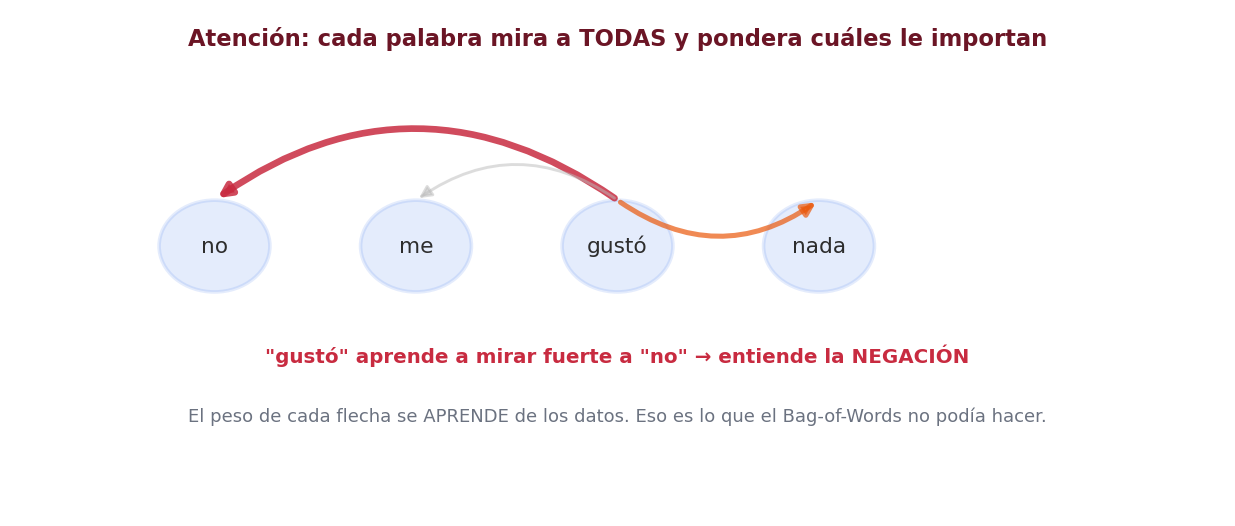
\includegraphics[width=0.78\textwidth]{fig_atencion_concepto.png}
  \end{center}
  \vspace{2pt}
  {\footnotesize\color{arcaDark}
  Para entender \textbf{``banco''} en \textit{``el banco del río crecio tras la lluvia''},
  la palabra mira a las demás. La atención mayor cae en \textbf{``río''} y la ambigüedad
  se resuelve: es la orilla. Cada palabra construye su significado \textbf{en contexto}.}
\end{frame}

\begin{frame}[shrink]{Por dentro --- Query, Key, Value (la metáfora del archivo)}
  \begin{columns}[c]
    \begin{column}{0.55\textwidth}
      \begin{center}
      \begin{tikzpicture}[font=\scriptsize, node distance=0.35cm]
        % contexto arriba
        \node[fill=arcaDark, text=white, rounded corners=4pt, align=center,
              minimum width=6cm, minimum height=0.8cm, font=\bfseries\footnotesize]
              (ctx) {frase: \itshape el banco del río creció};
        % tarjeta Q
        \node[rectangle, rounded corners=4pt, draw=arcaDark, fill=codeBlue!20,
              minimum width=6cm, minimum height=0.7cm, below=0.35cm of ctx,
              align=left, inner sep=5pt]
              (q) {\textbf{\color{codeBlue}Q}\;\, ``banco'' pregunta:\; \itshape¿qué me importa?};
        % tarjeta K
        \node[rectangle, rounded corners=4pt, draw=arcaDark, fill=codeOrange!20,
              minimum width=6cm, minimum height=0.7cm, below=0.2cm of q,
              align=left, inner sep=5pt]
              (k) {\textbf{\color{codeOrange}K}\;\, cada palabra ofrece:\; \itshape el, del, río, creció};
        % tarjeta V
        \node[rectangle, rounded corners=4pt, draw=arcaDark, fill=codeGreen!20,
              minimum width=6cm, minimum height=0.7cm, below=0.2cm of k,
              align=left, inner sep=5pt]
              (v) {\textbf{\color{codeGreen}V}\;\, info que cada una aporta};
        % barra de atención (resultado) - barra única ponderada
        \node[below=0.5cm of v, font=\bfseries\scriptsize\color{arcaDark}]
              (lbl) {atención de ``banco'' $\to$ cada palabra:};
        \begin{scope}[shift={($(lbl.south)+(-2.3,-0.3)$)}, every node/.style={font=\tiny}]
          \fill[codeBlue!40, draw=arcaDark] (0.0,0) rectangle (1.0,0.18);
          \fill[codeBlue!40, draw=arcaDark] (1.1,0) rectangle (2.1,0.27);
          \fill[arcaRed,     draw=arcaDark] (2.2,0) rectangle (3.2,0.90);
          \fill[codeBlue!40, draw=arcaDark] (3.3,0) rectangle (4.3,0.33);
          \node at (0.5,-0.2)  {el};
          \node at (1.6,-0.2)  {del};
          \node[font=\tiny\bfseries\color{arcaDark}] at (2.7,-0.2) {río};
          \node at (3.8,-0.2)  {creció};
          \node[font=\tiny\bfseries\color{arcaRed}] at (2.7, 1.05) {60\%};
        \end{scope}
      \end{tikzpicture}
      \end{center}
    \end{column}
    \begin{column}{0.45\textwidth}
      \vspace{2pt}
      \begin{itemize}\setlength{\itemsep}{6pt}
        \footnotesize
        \item \textbf{\color{codeBlue}Query} ($Q$):
        ``¿qué estoy buscando?''
        \item \textbf{\color{codeOrange}Key} ($K$):
        ``¿qué tengo para ofrecer?''
        \item \textbf{\color{codeGreen}Value} ($V$):
        ``¿qué información aporto?''
      \end{itemize}
      \vspace{6pt}
      \begin{tcolorbox}[colback=arcaGray, colframe=arcaRed, leftrule=3pt,
        boxrule=0pt, sharp corners, left=6pt, right=6pt, top=4pt, bottom=4pt]
        {\scriptsize\color{arcaDark}
        Como buscar un libro: tu \emph{query} es ``recetas de cocina'', la \emph{key}
        de cada libro es su título; donde matchea, tomas su \emph{value}.
        Pero \textbf{ponderado}, no de a uno --- aquí ``banco'' apuesta el 60\% a ``río''.}
      \end{tcolorbox}
    \end{column}
  \end{columns}
\end{frame}

\begin{frame}[shrink]{Multi-head --- varias cabezas, varias preguntas}
  \vspace{2pt}
  \begin{center}
  \begin{tikzpicture}[font=\footnotesize, node distance=0.4cm]
    \node[boxA, minimum width=2.6cm, align=center] (in) {entrada:\\una frase};
    \node[boxRed,    right=1.4cm of in.east, anchor=west, minimum width=2.4cm] (h1) {cabeza 1};
    \node[boxBlue,   below=0.5cm of h1, minimum width=2.4cm] (h2) {cabeza 2};
    \node[boxOrange, below=0.5cm of h2, minimum width=2.4cm] (h3) {cabeza 3};
    \node[font=\tiny\itshape\color{textMuted}, right=0.1cm of h1] {mira sintaxis};
    \node[font=\tiny\itshape\color{textMuted}, right=0.1cm of h2] {mira negación};
    \node[font=\tiny\itshape\color{textMuted}, right=0.1cm of h3] {mira sujeto};
    \node[fill=arcaDark, text=white, rounded corners, font=\bfseries\scriptsize,
          align=center, right=3.4cm of h2, anchor=west,
          minimum width=2.4cm, minimum height=1cm]
          (mix) {concatenar\\y combinar};
    \node[boxGreen, right=0.5cm of mix, align=center] (out) {salida\\enriquecida};
    \draw[arrowR] (in.east) -- (h1.west); \draw[arrowR] (in.east) -- (h2.west);
    \draw[arrowR] (in.east) -- (h3.west);
    \draw[arrowR] (h1.east) -- (mix.west); \draw[arrowR] (h2.east) -- (mix.west);
    \draw[arrowR] (h3.east) -- (mix.west);
    \draw[arrowR] (mix) -- (out);
  \end{tikzpicture}
  \end{center}
  \vspace{8pt}
  {\footnotesize\color{arcaDark}
  Cada \textbf{head} (cabeza) es una atención independiente que aprende a fijarse
  en algo distinto. BETO tiene \textbf{12 cabezas} por capa $\times$ 12 capas $=$
  \textbf{144 atenciones diferentes} mirando la frase en paralelo.}
\end{frame}

\begin{frame}[shrink]{Positional encoding --- meterle el orden de vuelta}
  \vspace{2pt}
  \begin{tcolorbox}[colback=arcaRed!8, colframe=arcaRed, leftrule=3pt,
    boxrule=0pt, sharp corners, left=8pt, right=8pt, top=4pt, bottom=4pt]
    {\footnotesize\color{arcaDark}\bfseries
    Problema: si todo se procesa en paralelo, el modelo no sabe el orden de las palabras.
    \textit{``perro muerde hombre''} y \textit{``hombre muerde perro''} le dan lo mismo.}
  \end{tcolorbox}
  \vspace{8pt}
  \begin{tcolorbox}[colback=arcaGray, colframe=arcaRed, leftrule=3pt,
    boxrule=0pt, sharp corners, left=8pt, right=8pt, top=6pt, bottom=6pt]
    {\footnotesize\color{arcaDark}
    \textbf{Solución del paper:} a cada vector de palabra se le \textbf{suma una firma
    de posición} (un patrón senoidal único para cada posición).\par
    \vspace{4pt}
    \[
      \text{entrada}_t \;=\; \underbrace{\text{embedding(palabra)}}_{\text{qué dice}}
      \;+\; \underbrace{\text{PE}(t)}_{\text{dónde está}}
    \]
    Así el modelo recupera el orden \emph{sin sacrificar el paralelismo}.}
  \end{tcolorbox}
\end{frame}

\begin{frame}[shrink]{La arquitectura completa del Transformer}
  \begin{center}
    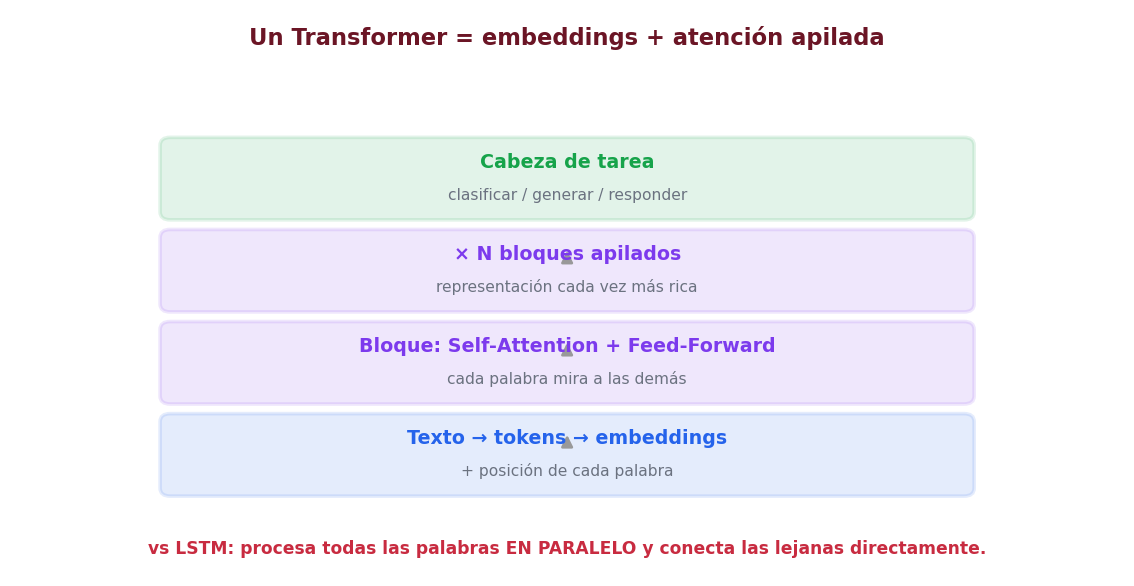
\includegraphics[width=0.42\textwidth]{fig_transformer_arquitectura.png}
  \end{center}
  \vspace{2pt}
  {\footnotesize\color{arcaDark}
  \textbf{Encoder} (izquierda): lee la entrada, aplica atención $N$ veces,
  produce una representación rica. \textbf{Decoder} (derecha): genera la salida
  token a token, atendiendo a su propio pasado y al encoder. BERT usa solo encoder;
  GPT usa solo decoder.}
\end{frame}

\begin{frame}[shrink]{Por qué cambió TODO --- tres propiedades}
  \begin{center}
  \begin{tikzpicture}[font=\footnotesize, node distance=0.3cm and 0.4cm]
    \node[boxRed, minimum width=4cm, minimum height=1.5cm, align=center] (p)
      {\textbf{\faRocket{} Paraleliza}\\\tiny procesa todas las palabras a la vez};
    \node[boxRed, right=of p, minimum width=4cm, minimum height=1.5cm, align=center] (m)
      {\textbf{\faBrain{} Memoria total}\\\tiny cualquier palabra alcanza a cualquier otra};
    \node[boxRed, right=of m, minimum width=4cm, minimum height=1.5cm, align=center] (s)
      {\textbf{\faChartLine{} Escala bien}\\\tiny más datos + parámetros = mejora};
  \end{tikzpicture}
  \end{center}
  \vspace{8pt}
  \begin{tcolorbox}[colback=arcaGray, colframe=arcaRed, leftrule=3pt,
    boxrule=0pt, sharp corners, left=8pt, right=8pt, top=4pt, bottom=4pt]
    {\footnotesize\color{arcaDark}
    Estas tres propiedades juntas posibilitaron entrenar modelos \emph{gigantes} sobre
    \emph{todo internet}. Sin ellas, GPT-3 (175 mil millones de parámetros) hubiera tardado
    \textbf{décadas} en entrenarse. Con ellas tardó semanas.}
  \end{tcolorbox}
\end{frame}

\begin{frame}[shrink]{Lo que el Transformer hizo posible}
  \begin{center}
    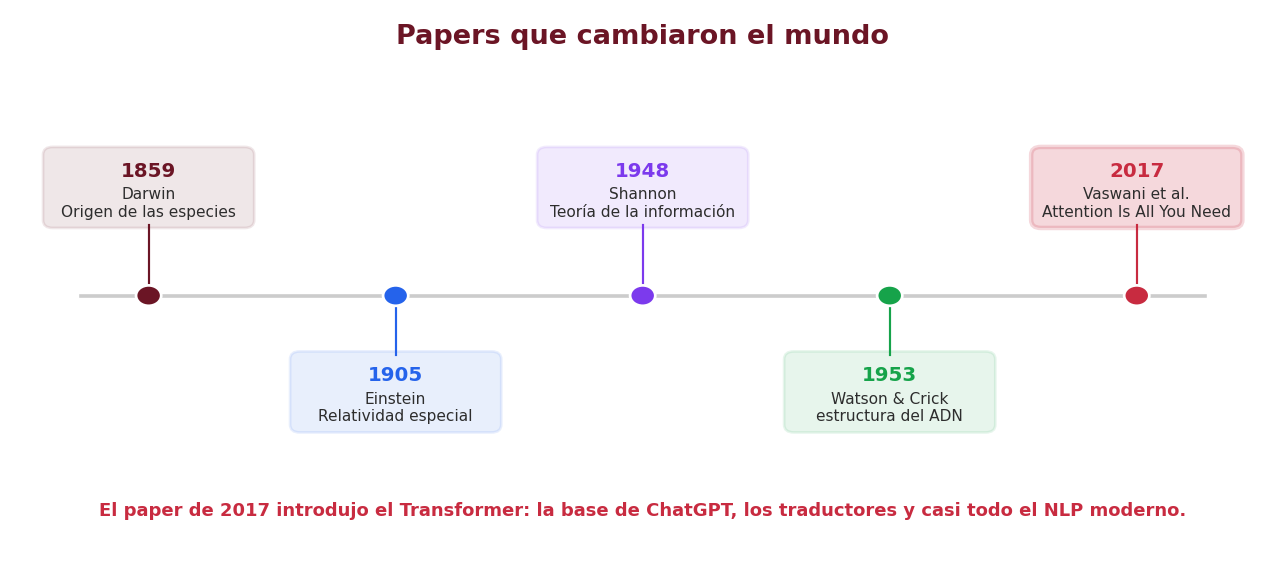
\includegraphics[width=0.85\textwidth]{fig_papers_historia.png}
  \end{center}
  \vspace{2pt}
  {\footnotesize\color{arcaDark}
  \textbf{2018:} BERT (Google) y GPT-1 (OpenAI) --- primeros Transformers gigantes
  pre-entrenados. \textbf{2020:} GPT-3, 175B params. \textbf{2022:} ChatGPT lo hace
  masivo. \textbf{2024--2026:} Claude, Gemini, Llama 4 --- la nueva normalidad.}
\end{frame}

\begin{frame}[shrink]{\faIndustry\ ¿Qué me llevo a Arca? --- Bloque 2}
  \vspace{4pt}
  {\footnotesize\color{arcaDark}\bfseries El lunes ya puedes:\par}
  \vspace{4pt}
  \begin{itemize}\setlength{\itemsep}{4pt}
    \footnotesize
    \item Cuando un proveedor te ofrezca ``IA con Transformers'', \textbf{ya sabes preguntar}:
    ¿pre-entrenado en español? ¿qué \emph{ventana de contexto}? ¿\emph{encoder} (BERT, búsqueda)
    o \emph{decoder} (GPT, generación)?
    \item Para procesar \textbf{documentos largos} (auditorías, contratos, manuales),
    elige modelos con \textbf{ventana de contexto grande} --- la atención es la razón por la
    que un LLM ``se acuerda'' del inicio del PDF.
    \item \textbf{No vas a entrenar atención. Vas a consumirla.} El oficio nuevo es saber
    elegir qué modelo, no programarlo desde cero.
  \end{itemize}
  \vspace{6pt}
  \begin{tcolorbox}[colback=arcaGray, colframe=arcaRed, leftrule=3pt,
    boxrule=0pt, sharp corners, left=8pt, right=8pt, top=4pt, bottom=4pt]
    {\footnotesize\color{arcaDark}\bfseries
    Nuestra pregunta: \emph{¿cómo entender el lenguaje de Arca sin contratar 50 lingüistas?}
    \faArrowRight\;Tercera respuesta: no entrenar --- usar uno que ya leyó todo el español.}
  \end{tcolorbox}
\end{frame}

% =============================================================================
%  BLOQUE 3 - MINI-TRANSFORMER EN ACCION
% =============================================================================
\sectionframe{Bloque 3}{Mini-Transformer en acción\\(spoiler: desde cero no funciona)}

\begin{frame}[shrink]{¿Y si entrenamos uno desde cero sobre muchocine?}
  \vspace{2pt}
  \begin{tcolorbox}[colback=arcaGray, colframe=arcaRed, leftrule=3pt,
    boxrule=0pt, sharp corners, left=8pt, right=8pt, top=4pt, bottom=4pt]
    {\footnotesize\color{arcaDark}
    Tenemos las 2.620 reseñas de \texttt{muchocine} de la clase pasada y el baseline
    TF-IDF+LogReg en \textbf{84\%}. ¿Qué pasa si reemplazamos el clasificador por un
    \textbf{Transformer encoder} entrenado desde cero?\par}
  \end{tcolorbox}
  \vspace{8pt}
  \begin{center}
  \begin{tikzpicture}[font=\scriptsize, node distance=0.25cm]
    \node[boxA] (in)  {tokens};
    \node[boxBlue, below=of in]  (emb) {Embedding + PE};
    \node[boxRed, below=of emb]  (b1)  {bloque MHA + FFN};
    \node[boxOrange, below=of b1] (pool){GlobalAvgPool};
    \node[boxGreen, below=of pool] (out) {Dense $\to$ POS/NEG};
    \draw[arrowR] (in)--(emb); \draw[arrowR] (emb)--(b1);
    \draw[arrowR] (b1)--(pool); \draw[arrowR] (pool)--(out);
    \node[right=1cm of b1, text width=6cm, font=\scriptsize, color=arcaDark]
      {\textbf{Mini-Transformer encoder}\\
       1 bloque, 2 cabezas, $\sim$300\,K parámetros, 10 épocas en GPU.\\
       Variante chica del paper, hecho a la medida del dataset.};
  \end{tikzpicture}
  \end{center}
\end{frame}

\begin{frame}[shrink]{Resultado --- el Transformer no aprende}
  \vspace{4pt}
  \begin{center}
  \begin{tabular}{lr}
    \toprule
    \textbf{Modelo} & \textbf{Accuracy validación}\\
    \midrule
    \rowcolor{arcaGray}
    TF-IDF + Regresión Logística & \textbf{84.4\%}\\
    Mini-Transformer (desde cero) & \color{arcaRed}\textbf{51.5\%} (azar = 50\%)\\
    \bottomrule
  \end{tabular}
  \end{center}
  \vspace{10pt}
  \begin{tcolorbox}[colback=arcaRed!8, colframe=arcaRed, leftrule=3pt,
    boxrule=0pt, sharp corners, left=8pt, right=8pt, top=6pt, bottom=6pt]
    {\footnotesize\color{arcaDark}\bfseries
    El Transformer no convergió. Con 2.620 reseñas no le alcanzaron los datos
    para que la atención significara algo: predijo \emph{todo igual}. La regla del
    oficio: un Transformer tiene cientos de miles de parámetros que ajustar, y
    necesita ver \textbf{millones} de frases para encontrar patrones útiles.}
  \end{tcolorbox}
  \vspace{6pt}
  \begin{tcolorbox}[colback=arcaGray, colframe=arcaRed, leftrule=3pt,
    boxrule=0pt, sharp corners, left=8pt, right=8pt, top=4pt, bottom=4pt]
    {\footnotesize\color{arcaDark}
    \faLightbulb~Esta es \textbf{la lección}. La pregunta inmediata: \emph{¿entonces
    quién entrena estos Transformers?} \textbf{Otros}. Y nosotros los usamos.}
  \end{tcolorbox}
\end{frame}

\begin{frame}[shrink]{La solución --- usar uno pre-entrenado (BETO)}
  \vspace{4pt}
  \begin{tcolorbox}[colback=arcaGray, colframe=arcaRed, leftrule=3pt,
    boxrule=0pt, sharp corners, left=8pt, right=8pt, top=6pt, bottom=6pt]
    {\footnotesize\color{arcaDark}
    \textbf{BETO} --- un BERT entrenado por la \textbf{Universidad de Chile} sobre
    \emph{toda} la Wikipedia en español + libros + noticias ($\sim$3 mil millones
    de palabras). \textbf{110 millones de parámetros}, descarga libre.}
  \end{tcolorbox}
  \vspace{8pt}
  \begin{center}
  \begin{tikzpicture}[font=\footnotesize, node distance=0.4cm]
    \node[boxA] (us)  {nuestro\\mini\\$\sim$100\,K};
    \node[fill=arcaRed!20, draw=arcaDark, rounded corners=4pt, font=\bfseries\footnotesize,
          right=1cm of us, minimum width=2.6cm, minimum height=1.3cm, align=center]
      (beto) {BETO\\110\,M params\\3\,B palabras};
    \node[font=\scriptsize\color{arcaDark}, below=0.1cm of beto] {U. de Chile};
    \node[font=\Large, right=0.5cm of beto] (eq) {=};
    \node[fill=codeGreen!20, draw=arcaDark, rounded corners=4pt, right=0.5cm of eq,
          minimum width=4.6cm, minimum height=1.3cm, align=center, font=\footnotesize]
      (pwr) {ya \emph{sabe} español\\porque le hicieron leer todo};
  \end{tikzpicture}
  \end{center}
  \vspace{6pt}
  {\footnotesize\color{arcaDark}
  Cargamos BETO y \emph{sin entrenar nada}, le mostramos \textit{``no me gustó nada
  la trama''}. ¿Qué ve por dentro?}
\end{frame}

\begin{frame}[shrink]{La atención de BETO sobre la negación}
  \begin{center}
    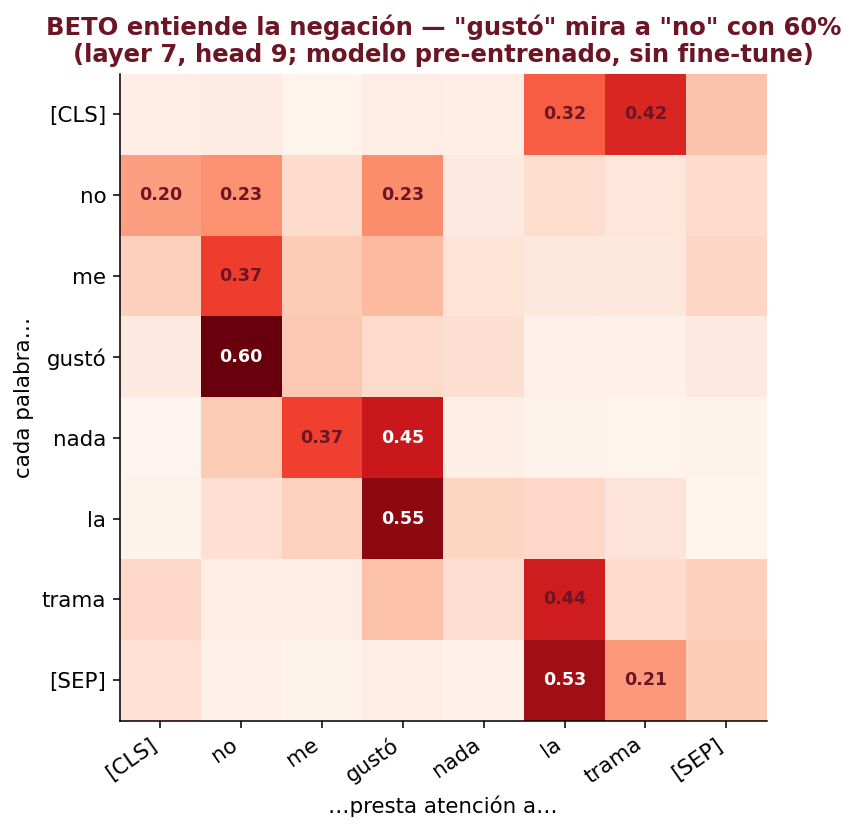
\includegraphics[height=0.66\textheight, keepaspectratio]{fig_attention_beto.png}
  \end{center}
  \vspace{-2pt}
  \begin{tcolorbox}[colback=arcaRed!8, colframe=arcaRed, leftrule=3pt,
    boxrule=0pt, sharp corners, left=8pt, right=8pt, top=4pt, bottom=4pt]
    {\footnotesize\color{arcaDark}\bfseries
    ``gustó'' presta \textbf{60\%} de su atención a ``no''. BETO lo aprendió pre-entrenando
    sobre miles de millones de palabras --- nadie se lo enseñó. \textbf{TF-IDF jamás podría.}}
  \end{tcolorbox}
\end{frame}

\begin{frame}[shrink]{Las 12 cabezas miran cosas distintas}
  \begin{center}
    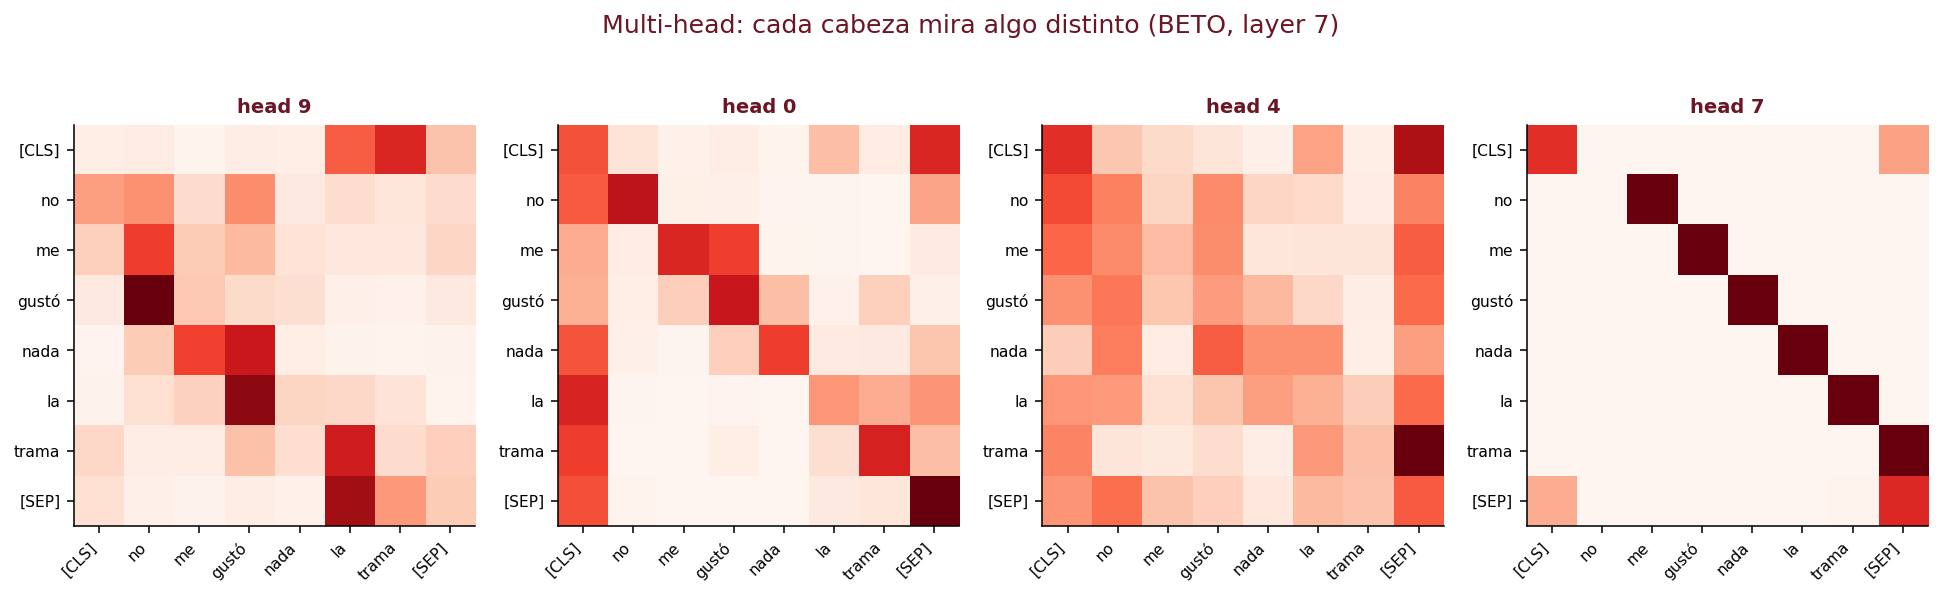
\includegraphics[width=0.95\textwidth]{fig_attention_heads.png}
  \end{center}
  \vspace{2pt}
  {\footnotesize\color{arcaDark}
  Algunas cabezas conectan negación con adjetivos, otras miran al \texttt{[CLS]} de
  contexto global, otras siguen patrones sintácticos. \textbf{144 perspectivas
  distintas} mirando la misma frase en paralelo.}
\end{frame}

\begin{frame}[shrink]{\faIndustry\ ¿Qué me llevo a Arca? --- Bloque 3}
  \vspace{4pt}
  {\footnotesize\color{arcaDark}\bfseries El lunes ya puedes:\par}
  \vspace{4pt}
  \begin{itemize}\setlength{\itemsep}{4pt}
    \footnotesize
    \item Para clasificar \textbf{quejas de consumidor en español}, \textbf{BETO con
    fine-tuning} de 2000 ejemplos etiquetados supera a TF-IDF y corre \emph{on-prem}.
    \item \textbf{Nunca entrenes un Transformer desde cero} con menos de 100k ejemplos
    --- es tirar plata. Empieza siempre por uno pre-entrenado.
    \item Si tu dato es \textbf{sensible y no puede salir de Arca}, \emph{BETO/Llama on-prem}
    es la respuesta, no la API pública de OpenAI.
  \end{itemize}
  \vspace{8pt}
  \begin{tcolorbox}[colback=arcaRed!8, colframe=arcaRed, leftrule=3pt,
    boxrule=0pt, sharp corners, left=8pt, right=8pt, top=6pt, bottom=6pt]
    {\small\color{arcaDark}\bfseries
    Nuestra pregunta: \emph{¿cómo entender el lenguaje de Arca sin contratar 50 lingüistas?}
    \faArrowRight\;Cuarta respuesta (último bloque): 5 líneas de Python y un API key.}
  \end{tcolorbox}
\end{frame}

% =============================================================================
%  BLOQUE 4 - LLMs + GROQ
% =============================================================================
\sectionframe{Bloque 4}{LLMs en la práctica:\\panorámica + 5 líneas de Python}

\begin{frame}[shrink]{¿Qué es un LLM, en una línea?}
  \vspace{14pt}
  \begin{center}
  \begin{tcolorbox}[colback=arcaGray, colframe=arcaRed, sharp corners,
    leftrule=4pt, boxrule=0pt, left=14pt, right=14pt, top=8pt, bottom=8pt,
    width=0.88\textwidth]
    {\large\color{arcaDark}\bfseries
    Un Transformer enorme entrenado para \textbf{predecir el siguiente token}\\
    sobre billones de palabras de internet.\par}
  \end{tcolorbox}
  \end{center}
  \vspace{14pt}
  {\footnotesize\color{arcaDark}
  Y eso es \textbf{exactamente} lo que hacía nuestro char-LSTM del Bloque 1 ---
  \textbf{predecir el siguiente carácter} y realimentarlo --- pero con tres diferencias:}
  \vspace{4pt}
  \begin{itemize}\setlength{\itemsep}{2pt}
    \footnotesize
    \item Predice el siguiente \textbf{token} (un fragmento de palabra, no carácter).
    \item Usa \textbf{atención} en lugar de recurrencia.
    \item Está entrenado sobre \textbf{escala bestial} (todo internet, miles de GPUs).
  \end{itemize}
\end{frame}

\begin{frame}[shrink]{El arco completo --- de Cervantes a ChatGPT}
  \begin{center}
  \begin{tikzpicture}[font=\footnotesize, node distance=0.3cm and 0.6cm]
    \node[fill=codeBlue!20, draw=arcaDark, rounded corners=5pt,
          minimum width=3.4cm, minimum height=1.7cm, align=center] (cl)
      {\bfseries char-LSTM\\del Bloque 1\\\tiny 350\,K params\\2\,MB Quijote};
    \node[fill=codePurple!20, draw=arcaDark, rounded corners=5pt, right=of cl,
          minimum width=3.4cm, minimum height=1.7cm, align=center] (mt)
      {\bfseries mini-Trans\\del Bloque 3\\\tiny 300\,K params\\desde cero, falla};
    \node[fill=arcaRed!20, draw=arcaDark, rounded corners=5pt, right=of mt,
          minimum width=3.4cm, minimum height=1.7cm, align=center] (be)
      {\bfseries BETO\\(pre-entrenado)\\\tiny 110\,M params\\3\,B palabras};
    \node[fill=arcaRed, text=white, draw=arcaDark, rounded corners=5pt, right=of be,
          minimum width=3.4cm, minimum height=1.7cm, align=center,
          font=\bfseries\footnotesize] (gpt)
      {GPT-5 / Claude\\\tiny 1\,T+ params\\todo internet};
    \draw[arrowR] (cl) -- (mt); \draw[arrowR] (mt) -- (be); \draw[arrowR] (be) -- (gpt);
  \end{tikzpicture}
  \end{center}
  \vspace{6pt}
  \begin{tcolorbox}[colback=arcaRed!8, colframe=arcaRed, leftrule=3pt,
    boxrule=0pt, sharp corners, left=8pt, right=8pt, top=6pt, bottom=6pt]
    {\small\color{arcaDark}
    Si la receta es la misma, \textbf{¿por qué nosotros no entrenamos GPT-5?}\par
    \vspace{2pt}
    Porque son 1{,}8 \emph{billones} de parámetros $\times$ \$25M de cómputo.
    Lo que sí podemos hacer es \textbf{usarlo} ---
    y eso vale el siguiente bloque.}
  \end{tcolorbox}
\end{frame}

\begin{frame}[shrink]{La escala --- 7 órdenes de magnitud}
  \begin{center}
    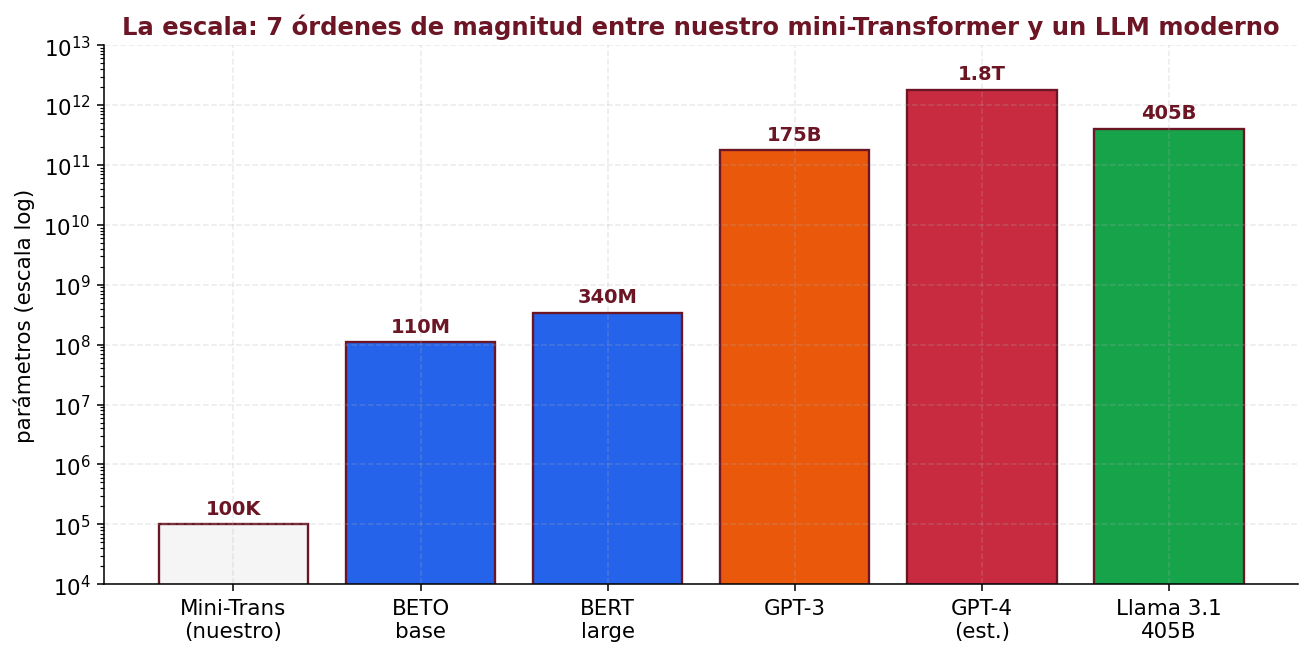
\includegraphics[width=0.86\textwidth]{fig_escala.png}
  \end{center}
  \vspace{2pt}
  {\footnotesize\color{arcaDark}
  Entre nuestro mini-Transformer ($100\,$K parámetros) y GPT-4 ($1{,}8$~trillones)
  hay un factor de \textbf{18 millones}. Pero la receta es la misma. Solo cambia
  la escala de datos y cómputo.}
\end{frame}

\begin{frame}[shrink]{El paradigma cambió --- de entrenar a USAR}
  \vspace{4pt}
  \begin{center}
  \begin{tikzpicture}[font=\footnotesize, node distance=0.3cm and 1.2cm]
    \node[fill=codeBlue!20, draw=arcaDark, rounded corners=4pt,
          minimum width=4.5cm, minimum height=2.5cm, align=center, text width=4.2cm]
          (a) {\bfseries ANTES (2010-2017)\\
            \tiny cada equipo entrenaba su modelo
            para su tarea, desde cero, con sus datos etiquetados};
    \node[fill=codeGreen!20, draw=arcaDark, rounded corners=4pt, right=of a,
          minimum width=4.5cm, minimum height=2.5cm, align=center, text width=4.2cm]
          (b) {\bfseries HOY (2020+)\\
            \tiny unos pocos laboratorios entrenan modelos gigantes (Meta, Google, OpenAI,
            Anthropic) y el resto los USA};
    \draw[arrowR, line width=2pt] (a) -- (b);
  \end{tikzpicture}
  \end{center}
  \vspace{8pt}
  \begin{tcolorbox}[colback=arcaRed!8, colframe=arcaRed, leftrule=3pt,
    boxrule=0pt, sharp corners, left=8pt, right=8pt, top=4pt, bottom=4pt]
    {\footnotesize\color{arcaDark}\bfseries
    Para Arca esto significa: tu equipo de datos rara vez va a entrenar un LLM
    desde cero (no tiene sentido económico). Va a saber \emph{elegir} uno y
    \emph{usarlo bien} --- ese es el oficio nuevo.}
  \end{tcolorbox}
\end{frame}

\begin{frame}[shrink]{El mapa del ecosistema 2026}
  \vspace{4pt}
  \begin{center}
  \begin{tikzpicture}[font=\scriptsize, node distance=0.2cm and 0.4cm]
    \draw[arcaDark, thick] (0,0) -- (12,0);
    \draw[arcaDark, thick] (6,-3.2) -- (6,3.2);
    \node[font=\bfseries\footnotesize, color=arcaDark, anchor=south] at (12.5, 0) {open source};
    \node[font=\bfseries\footnotesize, color=arcaDark, anchor=north] at (-0.5, 0) {propietario};
    \node[font=\bfseries\footnotesize, color=arcaDark, rotate=90, anchor=south] at (6, 3.4) {generalista};
    \node[font=\bfseries\footnotesize, color=arcaDark, rotate=90, anchor=north] at (6, -3.4) {especializado};

    % cuadrante propietario-generalista (sup. izq.)
    \node[boxRed] at (2.2, 2.5) {GPT-5};
    \node[fill=arcaRed!70, text=white, rounded corners, font=\bfseries\footnotesize,
          inner sep=5pt] at (3.7, 1.5) {Claude Sonnet 4.6};
    \node[fill=arcaRed!70, text=white, rounded corners, font=\bfseries\footnotesize,
          inner sep=5pt] at (1.9, 0.6) {Gemini 3 Pro};

    % cuadrante open source-generalista (sup. der.)
    \node[fill=codeGreen, text=white, rounded corners, font=\bfseries\footnotesize,
          inner sep=5pt] at (9.2, 2.5) {Llama 4 405B};
    \node[fill=codeGreen, text=white, rounded corners, font=\bfseries\footnotesize,
          inner sep=5pt] at (10, 1.5) {Mistral Large};
    \node[fill=codeGreen, text=white, rounded corners, font=\bfseries\footnotesize,
          inner sep=5pt] at (8.4, 0.6) {DeepSeek V4};

    % cuadrante propietario-especializado (inf. izq.)
    \node[fill=codePurple!80, text=white, rounded corners, font=\bfseries\footnotesize,
          inner sep=5pt] at (2.5, -1.7) {GPT-5 Code};

    % cuadrante open source-especializado (inf. der.)
    \node[fill=codeBlue, text=white, rounded corners, font=\bfseries\footnotesize,
          inner sep=5pt] at (9, -1.7) {BETO (español)};
  \end{tikzpicture}
  \end{center}
  \vspace{4pt}
  {\footnotesize\color{arcaDark}
  Cuatro cuadrantes según \textbf{quién es dueño} y \textbf{qué tan general}. Para
  datos sensibles de Arca, los \emph{open source} permiten correr en infraestructura
  propia. Para máxima calidad, los \emph{propietarios} en la frontera.}
\end{frame}

\begin{frame}[shrink]{Costos 2026 --- 100x entre el más barato y el más capaz}
  \begin{center}
    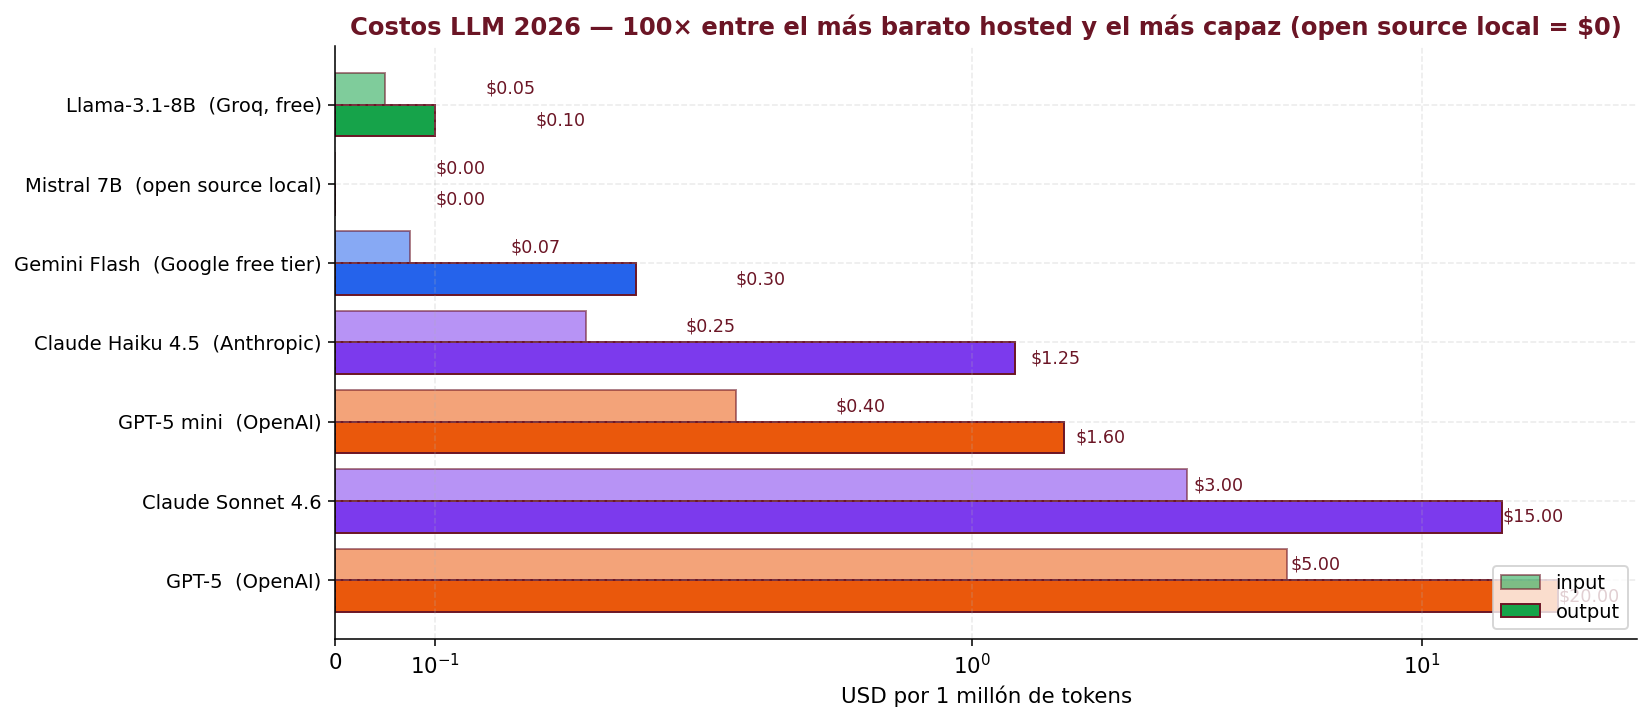
\includegraphics[width=0.88\textwidth]{fig_costos_llms.png}
  \end{center}
  \vspace{2pt}
  {\footnotesize\color{arcaDark}
  Para tareas masivas (clasificar 1M tickets), un \emph{open source} en Groq cuesta
  \$0.05/M tokens. Para tareas críticas (asistente legal), Claude Sonnet a \$15/M.
  La elección depende del valor de la tarea, no del prestigio del modelo.}
\end{frame}

\begin{frame}[shrink]{Cómo hablamos con un LLM --- la API REST}
  \begin{center}
  \begin{tikzpicture}[font=\footnotesize, node distance=0.4cm and 1.5cm]
    \node[boxBlue, minimum width=3cm, minimum height=1cm, align=center] (cli) {tu Python\\\tiny\bfseries cliente};
    \node[fill=arcaDark, text=white, rounded corners=4pt, right=of cli, align=center,
          minimum width=3cm, minimum height=1cm, font=\bfseries\footnotesize]
          (api) {endpoint HTTPS\\\tiny api.groq.com};
    \node[boxRed, right=of api, minimum width=3cm, minimum height=1cm, align=center] (mod) {modelo\\Llama 3.1};
    \draw[arrowR] (cli) -- (api);
    \draw[arrowR] (api) -- (mod);
    \node[font=\scriptsize\itshape\color{arcaDark}]
      at ($(cli.north)!0.5!(api.north)+(0,0.4)$) {prompt};
    \node[font=\scriptsize\itshape\color{arcaDark}]
      at ($(api.north)!0.5!(mod.north)+(0,0.4)$) {respuesta del modelo};
    \draw[arrowD, dashed] (mod.south) -- ++(0,-0.9) -| (cli.south);
    \node[font=\scriptsize\itshape\color{arcaDark}]
      at ($(cli.south)!0.5!(mod.south)+(0,-1.15)$) {respuesta JSON al cliente};
  \end{tikzpicture}
  \end{center}
  \vspace{8pt}
  \begin{tcolorbox}[colback=arcaGray, colframe=arcaRed, leftrule=3pt,
    boxrule=0pt, sharp corners, left=8pt, right=8pt, top=4pt, bottom=4pt]
    {\footnotesize\color{arcaDark}
    \textbf{Casi todos los proveedores hablan el mismo formato} (``OpenAI-compatible'').
    El código que usas para ChatGPT funciona, con un cambio de \texttt{base\_url},
    para Groq, Together, OpenRouter, Fireworks, vLLM local\dots}
  \end{tcolorbox}
\end{frame}

\begin{frame}[fragile, shrink]{La estructura del REQUEST --- qué le mandás al LLM}
  \vspace{2pt}
  \begin{pyblock}
request = {
    "model":       "llama-3.1-8b-instant",
    "messages": [
        {"role": "system", "content": "Eres asistente de planta de Arca."},
        {"role": "user",   "content": "Da 3 causas de vibracion de una llenadora."}
    ],
    "temperature": 0.3,
    "max_tokens":  300,
}
  \end{pyblock}
  \vspace{4pt}
  \begin{itemize}\setlength{\itemsep}{3pt}
    \footnotesize
    \item \texttt{model}: qué modelo del provider usás (\texttt{llama-3.1-8b-instant}, \texttt{llama-3.3-70b-versatile}\dots).
    \item \texttt{messages}: lista ordenada. \textbf{Roles}: \texttt{system} (instrucción de comportamiento),
    \texttt{user} (tu pregunta), \texttt{assistant} (respuestas previas en chat multi-turno).
    \item \texttt{temperature}: 0.0 determinista (clasificar, extraer) $\leftrightarrow$ 0.7+ creativo (escribir, sugerir).
    \item \texttt{max\_tokens}: tope de salida (cortar antes para limitar costo y latencia).
  \end{itemize}
  \vspace{2pt}
  \begin{tcolorbox}[colback=arcaRed!8, colframe=arcaRed, leftrule=3pt,
    boxrule=0pt, sharp corners, left=8pt, right=8pt, top=3pt, bottom=3pt]
    {\footnotesize\color{arcaDark}\bfseries
    Eso es \emph{todo} lo que viaja a un endpoint OpenAI-compatible.
    Es un POST con este JSON.}
  \end{tcolorbox}
\end{frame}

\begin{frame}[fragile, shrink]{La estructura del RESPONSE --- qué te devuelve el LLM}
  \vspace{2pt}
  \begin{pyblock}
response = {
    "id":      "chatcmpl-abc123",
    "model":   "llama-3.1-8b-instant",
    "choices": [
        {
            "index": 0,
            "message":       {"role": "assistant", "content": "1. Pernos sueltos..."},
            "finish_reason": "stop",
        }
    ],
    "usage": {
        "prompt_tokens":     42,
        "completion_tokens": 87,
        "total_tokens":      129,
    },
}
  \end{pyblock}
  \vspace{2pt}
  \begin{itemize}\setlength{\itemsep}{2pt}
    \footnotesize
    \item Lo que querés está en \texttt{response.choices[0].message.content}.
    \item \texttt{finish\_reason}: \texttt{stop} (terminó bien) vs \texttt{length} (se quedó sin tokens).
    \item \texttt{usage}: cuántos tokens consumiste (=~ \$). Útil para estimar costo en producción.
  \end{itemize}
  \vspace{2pt}
  \begin{tcolorbox}[colback=arcaGray, colframe=arcaRed, leftrule=3pt,
    boxrule=0pt, sharp corners, left=8pt, right=8pt, top=3pt, bottom=3pt]
    {\footnotesize\color{arcaDark}
    \textbf{Este JSON es el estándar.} Groq, OpenAI, Together, Fireworks, vLLM\dots
    todos te devuelven la \emph{misma forma}. Tu código de negocio NO cambia al cambiar
    de provider --- sólo el \texttt{base\_url} y el \texttt{api\_key}.}
  \end{tcolorbox}
\end{frame}

\begin{frame}[fragile, shrink]{El demo --- 5 líneas Python contra Groq}
  \begin{pyblock}
from openai import OpenAI
import os

client = OpenAI(api_key=os.environ["GROQ_API_KEY"],
                base_url="https://api.groq.com/openai/v1")

resp = client.chat.completions.create(
    model="llama-3.1-8b-instant",
    messages=[{"role": "user",
               "content": "Resume el mantenimiento de una llenadora en 3 viñetas."}],
)
print(resp.choices[0].message.content)
  \end{pyblock}
  \vspace{4pt}
  {\footnotesize\color{arcaDark}
  Eso es \textbf{todo}. Una API key gratuita en \texttt{console.groq.com} (sin tarjeta),
  10 segundos, y ya estás llamando a un Llama 3.1 de \textbf{8 mil millones de parámetros}
  desde tu portátil.}
\end{frame}

\begin{frame}[shrink]{La respuesta real --- generación, 1.97s, 360 tokens}
  \vspace{2pt}
  \begin{tcolorbox}[colback=arcaGray, colframe=codeGreen, leftrule=3pt,
    boxrule=0pt, sharp corners, left=8pt, right=8pt, top=4pt, bottom=4pt,
    title={\scriptsize\color{white}\bfseries Llama 3.1-8B en Groq},
    coltitle=white, colbacktitle=codeGreen, fonttitle=\scriptsize]
    {\scriptsize\color{textDark}
    Aquí te presento un plan de mantenimiento preventivo semanal para una llenadora
    industrial en una planta embotelladora:\par
    \vspace{2pt}
    \textbullet\ \textbf{Lunes: Verificación de la línea de llenado}\par
    \quad+ Verificar el estado de los tubos y conexiones de la línea de llenado.\par
    \quad+ Revisar la presión de los sistemas de bombeo y la estanqueidad de las válvulas.\par
    \quad+ Verificar la temperatura de los tanques de almacenamiento.\par
    \vspace{2pt}
    \textbullet\ \textbf{Miércoles: Mantenimiento de los sistemas de control}\par
    \quad+ Verificar la conectividad con la red de control.\par
    \quad+ Revisar la programación y configuración de los controles.\par
    \vspace{2pt}
    \textbullet\ \textbf{Viernes: Verificación de la limpieza y desinfección}\par
    \quad+ Verificar la limpieza de los tanques y la efectividad de la desinfección.}
  \end{tcolorbox}
  \vspace{4pt}
  {\footnotesize\color{arcaDark}
  Una respuesta estructurada, en español técnico, relevante al dominio.
  \textbf{No le entrenamos nada}; le hablamos en español y respondió.}
\end{frame}

\begin{frame}[shrink]{El mismo modelo también clasifica y extrae}
  \vspace{2pt}
  {\footnotesize\color{arcaDark}\textbf{Clasificación de sentimiento (0.34\,s, 115 tokens):}\par}
  \begin{tcolorbox}[colback=arcaGray, colframe=codeBlue, leftrule=3pt,
    boxrule=0pt, sharp corners, left=8pt, right=8pt, top=2pt, bottom=2pt]
    {\scriptsize\color{textDark}
    1. \textit{``no me gustó nada la trama''} \;\faArrowRight\; \textbf{\color{codeGreen}NEGATIVO} \faCheck\par
    2. \textit{``no es para nada mala, me sorprendió''} \;\faArrowRight\; \textbf{\color{codeGreen}POSITIVO} \faCheck\par
    3. \textit{``buena fotografía pero la historia no funciona''} \;\faArrowRight\; \textbf{\color{codeGreen}NEGATIVO} \faCheck}
  \end{tcolorbox}
  \vspace{6pt}
  {\footnotesize\color{arcaDark}\textbf{Extracción de un ticket de planta a JSON (0.9\,s, 147 tokens):}\par}
  \begin{tcolorbox}[colback=arcaGray, colframe=codeOrange, leftrule=3pt,
    boxrule=0pt, sharp corners, left=8pt, right=8pt, top=2pt, bottom=2pt]
    {\scriptsize\ttfamily\color{textDark}
    input:\;``El compresor número 3 está echando vapor desde anoche, urge revisión.''\par
    \vspace{2pt}
    output:\par
    \{\par
    \quad"equipo": "compresor número 3",\par
    \quad"problema": "echando vapor",\par
    \quad"urgencia": "alta"\par
    \}}
  \end{tcolorbox}
  \vspace{4pt}
  {\footnotesize\color{arcaDark}\bfseries
  El \emph{mismo} modelo, sin reentrenar nada, resuelve generación, clasificación
  y extracción estructurada. Esto antes era un proyecto de 6 meses cada uno.}
\end{frame}

\begin{frame}[shrink]{\faIndustry\ ¿Qué me llevo a Arca? --- Bloque 4 + Módulo 6}
  \vspace{4pt}
  {\footnotesize\color{arcaDark}\bfseries El lunes ya puedes:\par}
  \vspace{4pt}
  \begin{itemize}\setlength{\itemsep}{4pt}
    \footnotesize
    \item \textbf{3 tareas con la misma API key}: clasificar el backlog de tickets,
    extraer JSON estructurado del SAP, resumir reportes de turno.
    \item \textbf{Regla de costo}: tareas masivas ($>$10k req/día) $\to$ open source en Groq
    (\$0.05/M tok). Tareas críticas (legal, contratos) $\to$ Claude Sonnet (\$15/M tok).
    \textbf{No uses GPT-5 para clasificar emails.}
    \item Antes de pedir un proyecto de 6 meses: \textbf{prototipa en 1 día}
    con un Notebook + Groq. Si funciona, ya tienes el business case.
  \end{itemize}
  \vspace{8pt}
  \begin{tcolorbox}[colback=arcaRed!8, colframe=arcaRed, leftrule=3pt,
    boxrule=0pt, sharp corners, left=8pt, right=8pt, top=6pt, bottom=6pt]
    {\footnotesize\color{arcaDark}\bfseries
    \faArrowRight\;\textbf{Módulo 6} profundiza esto en hands-on: \emph{prompting} avanzado,
    \emph{RAG} con tus documentos, \emph{agentes} que actúan, \emph{web scraping} para
    alimentar todo, \emph{APIs en producción} (rate limits, costos, fallback).}
  \end{tcolorbox}
\end{frame}

% =============================================================================
%  CIERRE
% =============================================================================
\sectionframe{Cierre}{Lo que te llevas}

\begin{frame}[shrink]{La respuesta a la pregunta del día}
  \vspace{2pt}
  \begin{tcolorbox}[colback=arcaDark, colframe=arcaDark, sharp corners,
    boxrule=0pt, left=10pt, right=10pt, top=5pt, bottom=5pt]
    {\footnotesize\color{white}\itshape
    ¿Cómo le enseñamos a una máquina a entender el lenguaje de Arca ---
    manuales de mantenimiento, tickets de planta, quejas de consumidor ---
    sin contratar 50 lingüistas?\par}
  \end{tcolorbox}
  \vspace{6pt}
  \begin{tcolorbox}[colback=arcaRed!8, colframe=arcaRed, leftrule=3pt,
    boxrule=0pt, sharp corners, left=8pt, right=8pt, top=6pt, bottom=6pt]
    {\small\color{arcaDark}\bfseries
    No le enseñamos --- \emph{elegimos el modelo correcto y le hablamos en nuestro
    dominio}. El oficio nuevo es \textbf{elegir y orquestar}, no entrenar.}
  \end{tcolorbox}
  \vspace{4pt}
  {\footnotesize\color{arcaDark}\bfseries Cómo llegamos a esa respuesta:\par}
  \vspace{2pt}
  \begin{itemize}\setlength{\itemsep}{3pt}
    \footnotesize
    \item Antes de 2017, las LSTM tenían \textbf{3 muros}: secuencial, olvido, no escalan.
    \item ``Attention is All You Need'' (2017) propuso el \textbf{Transformer}: cada palabra
    mira a todas a la vez. \textbf{QKV + multi-head + positional encoding.}
    \item Entrenar uno desde cero requiere datos masivos (nuestro mini no aprendió).
    Un \textbf{pre-entrenado} (BETO) ya entiende español: \emph{gustó} $\to$ \emph{no} al 60\%.
    \item Un \textbf{LLM} es eso mismo a otra escala: GPT predice el siguiente token,
    igual que nuestro char-LSTM, pero con atención + escala bestial.
    \item En \textbf{5 líneas de Python} hablamos a un Llama 3.1 vía Groq. Módulo 6 profundiza.
  \end{itemize}
\end{frame}

\begin{frame}[plain, noframenumbering]
  \begin{tikzpicture}[remember picture, overlay]
    \fill[arcaDark] (current page.south west) rectangle (current page.north east);
    \node[anchor=center, text=white, font=\Huge\bfseries] at
      ([yshift=1cm]current page.center) {Gracias};
    \node[anchor=center, text=white!85, font=\Large] at
      ([yshift=-0.2cm]current page.center) {Preguntas?};
    \node[anchor=center, text=white!70, font=\small] at
      ([yshift=-1.5cm]current page.center)
      {Clase 34 --- Del LSTM al LLM};
    \node[anchor=center, text=white!60, font=\scriptsize] at
      ([yshift=-2cm]current page.center)
      {github.com/cmosquerat/arca-diplomado/tree/main/clase-34};
  \end{tikzpicture}
\end{frame}

\end{document}
